Ahora, con el dispositivo experimental debidamente estudiado, podemos utilizarlo para obtener información de las fibras. En primer lugar procedemos a obtener la desviación estadar debido a la posición de la fibra en el dispositivo experimental. 

La existencia de esta incertidumbre es debida a que los conectores, que se fijan a la fibra, son los que marcan la posición de esta en el dispositivo experimental ya que son los que encajan perfectamente en el colimador. Sin embargo estos conectores pueden estar más o menos cerca del extremo de la fibra. En otras palabras, una vez fijados los conectores en la fibra, su posición queda perfectamente determinada, sin embargo estos conectores no siempre se situan exactamente en la misma posición de la fibra. Se trata de desviaciones mínimas del orden de $1~\mm$.

Esta es una desviación inherente al dispositivo experimental, por lo que siempre se encuentra presente. Debido a ello, si queremos quantizar incertidumbres procedentes de otras fuentes será necesario, en primer lugar, quantizar esta incertidumbre para poder extraerla. 

El experimento que se diseñó para determinar esta incertidumbre consistía en preparar una fibra de una longitud de $200~\mm$, longitud activa que posee el detector de Tritium, introducirla en el dispositivo experimental, quitarla y repetir este proceso durante un número N de veces (en nuestro caso se realizo para N=10). 

Seguidamente, se alimentó la LED con una intensidad de $0.1~\milli\ampere$ y, para cada una de estas 10 repeticiones, se midió la intensidad con ayuda de un picoamperímetro el cual proporciona la media $I_i$ y error $\sigma_{i}$ de un número N de medidas (para nuestro casó se utilizó N=100).

Se realizó este estudio para fibras de cada uno de los tipos sometidos a estudio (no clad, single clad y multiclad). Los resultados de estos tres tipos pueden verse ordenados en un histograma en las figuras \ref{posnoclad}, \ref{possingleclad} y \ref{posmulticlad} respectivamente:

\begin{figure}[hbtp]
\centering
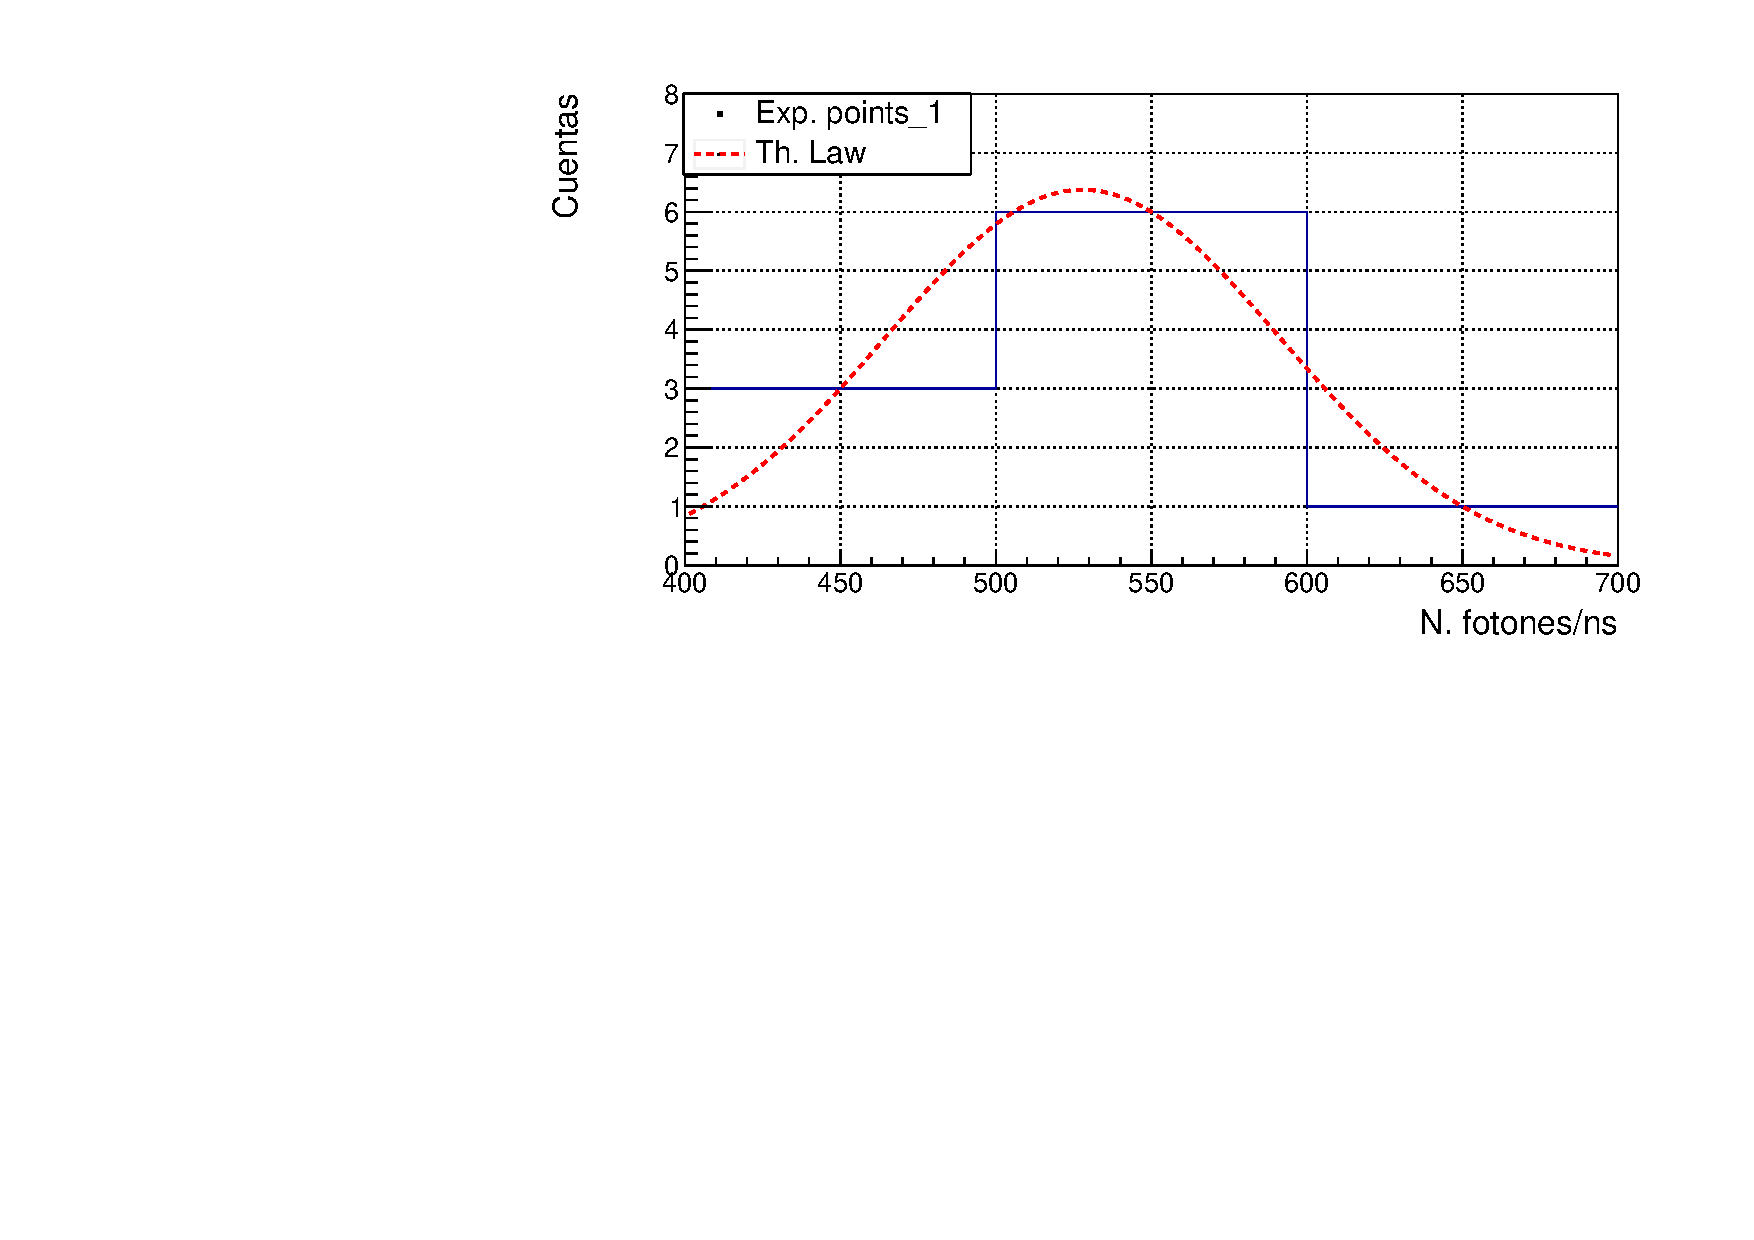
\includegraphics[scale=0.7]{Figuras/Nocladgauspos.pdf}
\caption{Histograma de las señales medidas para fibras no clad de 200 mm de longitud\label{posnoclad}}
\end{figure}

\begin{figure}[hbtp]
\centering
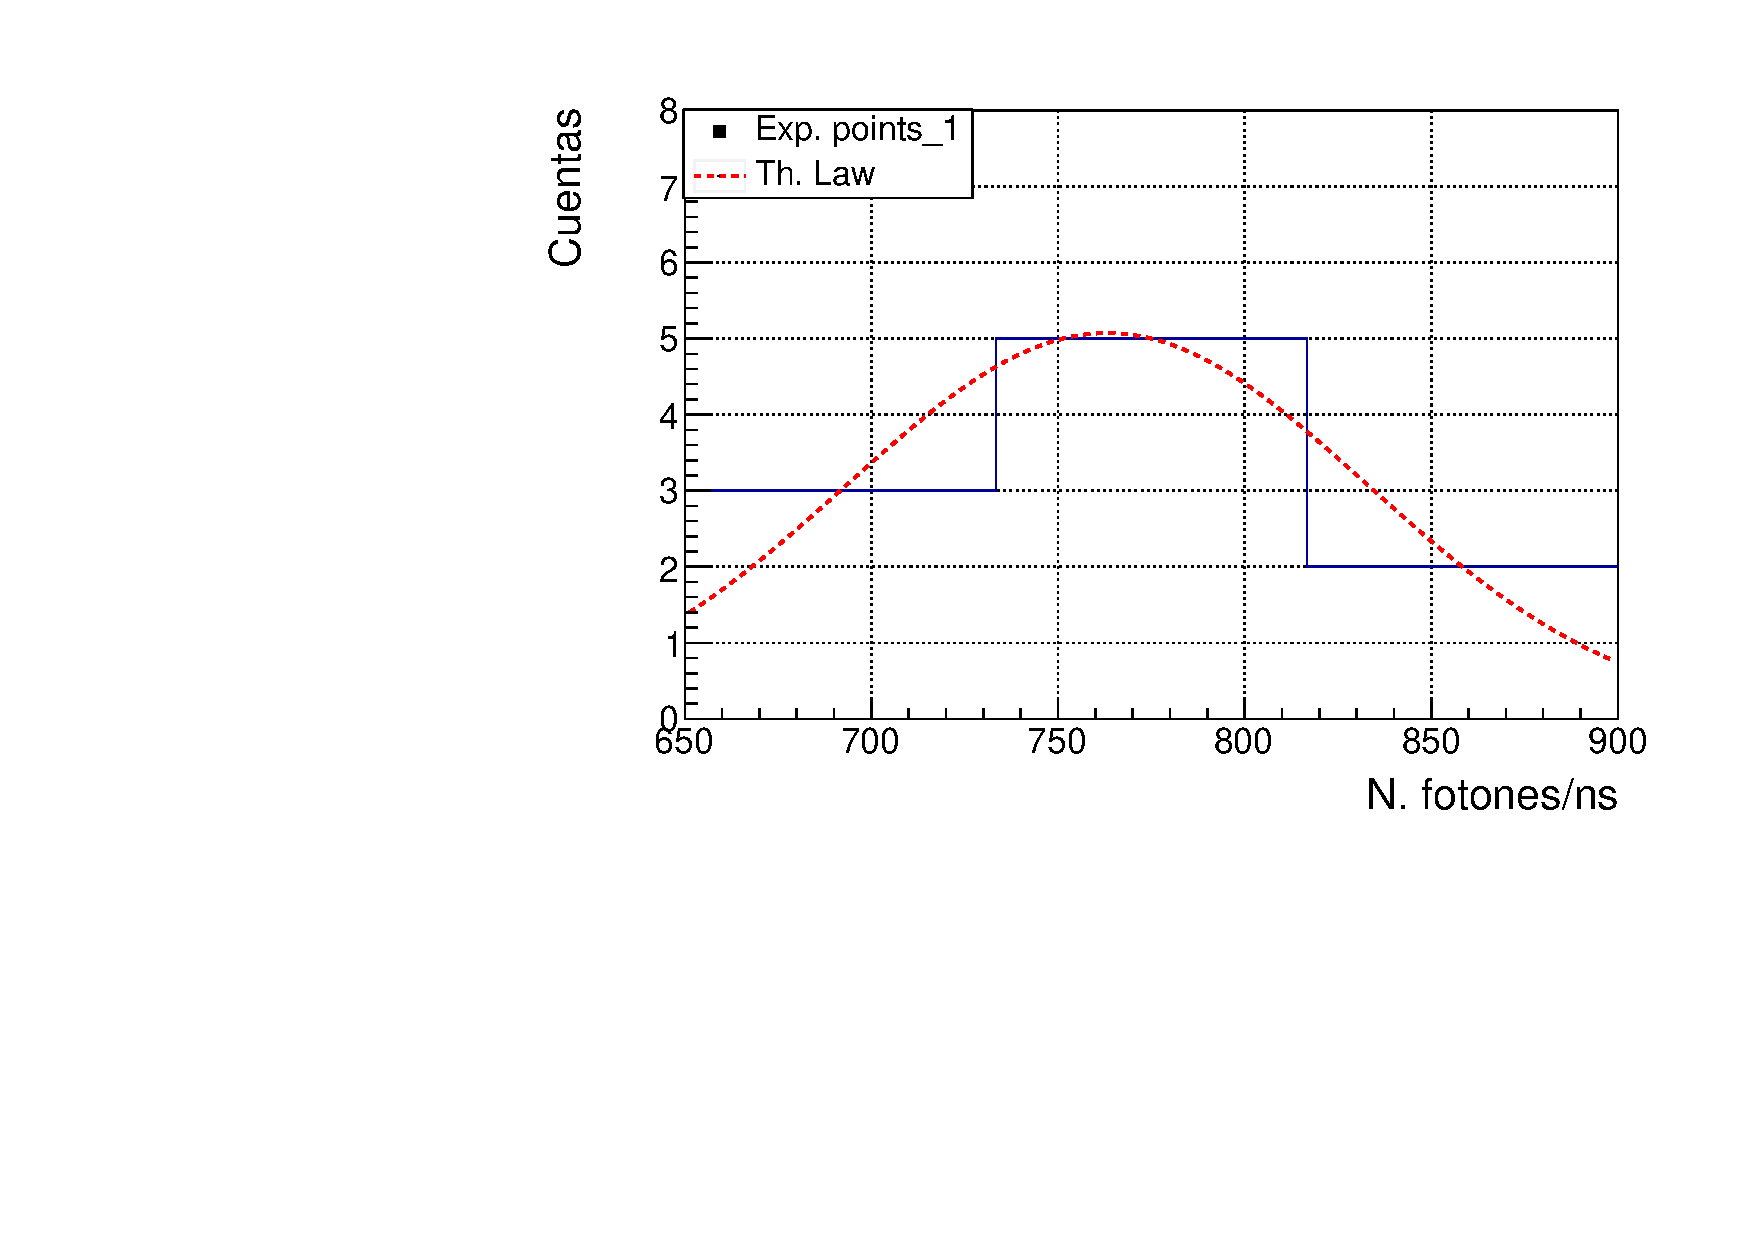
\includegraphics[scale=0.7]{Figuras/singlecladgauspos.pdf}
\caption{Histograma de las señales medidas para fibras single clad de 200 mm de longitud\label{possingleclad}}
\end{figure}

\begin{figure}[hbtp]
\centering
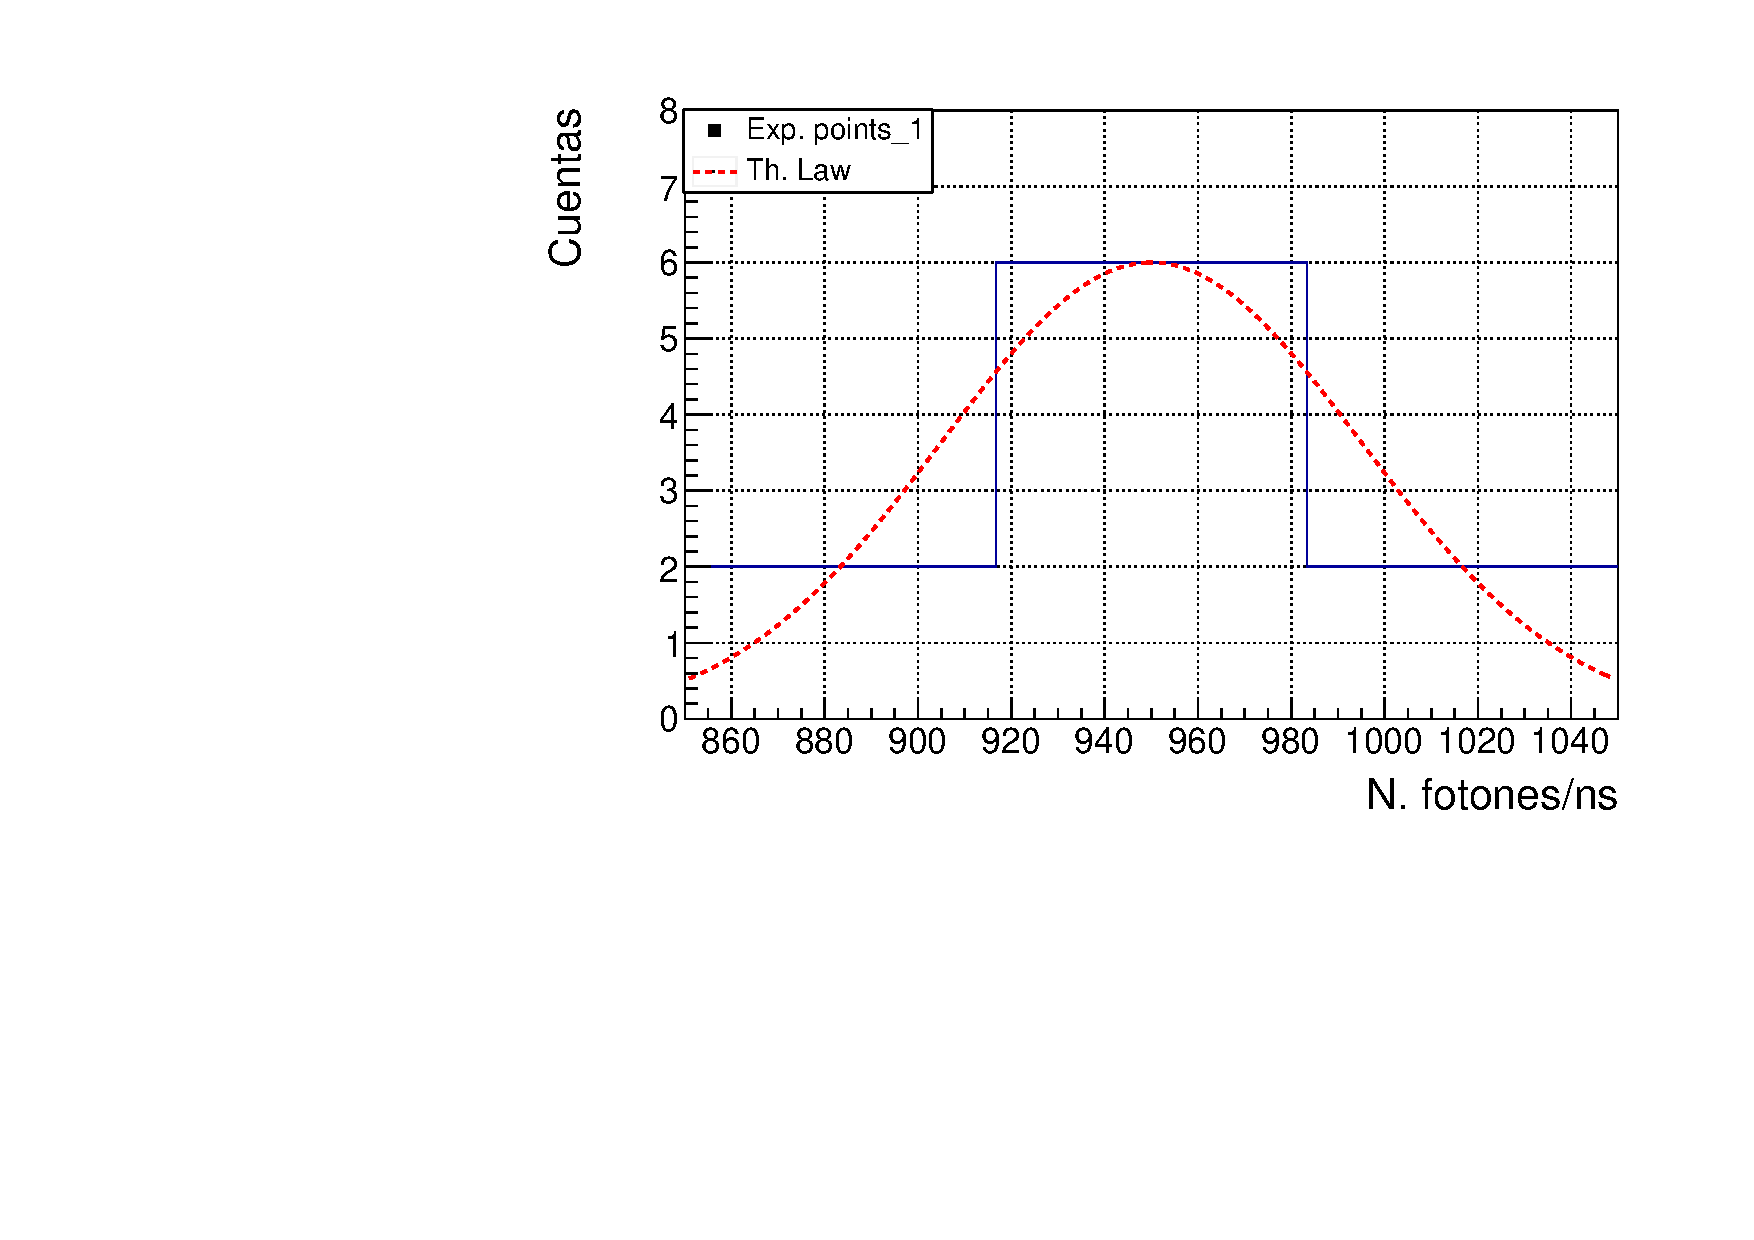
\includegraphics[scale=0.7]{Figuras/multicladgauspos.pdf}
\caption{Histograma de las señales medidas para fibras multi clad de 200 mm de longitud\label{posmulticlad}}
\end{figure}

Podemos observar que, como era de esperar, los resultados de cada experimento se distribuyen segun una gaussiana a la cual, se ha realizado un ajuste com opuede verse en las anteriores figuras \ref{posnoclad}, \ref{possingleclad} y \ref{posmulticlad}. Hay que tener en cuenta que, por el hecho de haber realizado el experimento para un número de repeticiones N relativamente bajo la resolución de esta gaussiana es mala.

Finalmente, para cada tipo de fibra, obtenemos la media y la desviación estandar según las expresiones \ref{ecuacionmedia} y \ref{ecuaciondesviacionestandar} respectivamente ya que este es un método más formal para un número de muestras N bajo:

\begin{equation}
\overline{x}=\sum_{i=1}^N \dfrac{x_i}{N}
\label{ecuacionmedia}
\end{equation}

\begin{equation}
\sigma=\dfrac{\sqrt{\sum_{i=1}^N (x_i-\overline{x})^2}}{N-1}
\label{ecuaciondesviacionestandar}
\end{equation}

Los valores obtenidos para cada tipo de fibra se muestran en la tabla \ref{tablasigmapos}

\begin{table}[H]
\begin{center}
\begin{tabular}{l | c | c | c | c }
Tipo de fibra & Media $(N.~\gamma/\nano\second)$ & Des. Std $(N.~\gamma/\nano\second)$ & Error $(N.~\gamma/\nano\second)$ & Des. Std. Rel\\
\hline \hline
No Clad & $524.09$ & $17.65$ & $0.010$ & $3.37$\\ 
Single clad & $765.63$ & $16.62$ & $0.012$ & $2.17$\\
Multi clad & $949.93$ & $9.91$ & $0.026$ & $1.04$\\
\end{tabular}
\caption{Resultado del estudio de la determinación de la desviación estandar debida a la posición de la fibra en el dispositivo experimental\label{tablasigmapos}}
\end{center}
\end{table}

En la tabla podemos observar que se a mostrado a demas una columna llamda "error". Este error es el obtenido por propagación del error aportado por el picoamperímetro en la medida, según se ha explicado antes. Los resultados que hemos sido capaces de determinar con este experimento son:

\begin{itemize}

\item{} Una medida del número de fotones por unidad de tiempo que cada tipo de fibra es capaz de recolectar para una misma intensidad de fotones a la entrada (la cual, si la conocemos, podríamos obtener la eficiencia absoluta de colección de luz de cada tipo de fibra). Podemos observar que esta recolección de luz es mayor a medida que aumenta el clad en la fibra, algo que cabría esperar ya que el principal objetivo de el clad es mejorar la colección de luz.

\item{} Una medida de la desviación estandar debida a la posición de la fibra en el dispositivo experimental para cada tipo de fibra, el cual era el objetivo inicial del estudio. Podemos observar que esta incertidumbre se mejora al añadir un primer cald y, esta mejora, se aumenta al añadir el segundo clad. Es decir, el cald no solo aporta una mejor recolección de luz, sino una mayor uniformidad en la señal obtenida ante lijeros desplazamientos de la fibra.

\item{} Se ha determinado por propagación el error experimental que asociado a la instrumentación empleada, el cual podemos observar que es tres órdenes de magnitud inferior a la desviación estandar, por lo que podemos despreciarlo en el estudio.

\item{} Finalmente se ha obtenido la desviación estandar relativa como el cociente entre la desviación estandar y la media. Podemos observar, como era de esperar, que este se reduce a medida que aumentamos el clad en la fibra.

\end{itemize}
